\chapter{Alberi Binari di Ricerca}
\thispagestyle{chapterInit}
\section{Alberi Binari di Ricerca}
    \paragraph{Dizionario} \begin{definition}
        Un \textbf{dizionario} è una struttura dati che implementa le seguenti funzionalità: 
        \begin{itemize}
            \item \texttt{Item lookup(Item k)}: restituisce l'elemento con chiave $k$ se presente nel dizionario.
            \item \texttt{insert(Item k, Item v)}: inserisce l'elemento $i$ con chiave $k$ e valore $v$ nel dizionario.
            \item \texttt{remove(Item k)}: elimina l'elemento con chiave $k$ dal dizionario.
        \end{itemize}
    \end{definition}
    \subparagraph{Possibili Implementazioni} di seguito sono riportate le possibili implementazioni di un dizionario:
        \begin{table}[H]
            \centering
            \begin{tabular}{|c|c|c|c|}
                \hline
                \textbf{Struttura} & \textbf{\texttt{lookup}} & \textbf{\texttt{insert}} & \textbf{\texttt{remove}} \\
                \hline
                Vettore Ordinato & $O(\log n)$ & $O(n)$ & $O(n)$ \\
                \hline
                Vettore non Ordinato & $O(n)$ & $O(1)$* & $O(1)$* \\
                \hline
                Lista non Ordinata & $O(n)$ & $O(1)$ & $O(1)$* \\
                \hline
            \end{tabular}
        \end{table}
        * Assumendo che l'elemento sia già stato trovato, altrimenti $O(n)$.
    \paragraph{Idea ispiratrice} Portare l'idea di ricerca binaria negli alberi.
    \paragraph{Memorizzaione}\begin{itemize}
        \item Le \textbf{associazioni chiave-valore} vengono memorizzate in un albero binario
        \item Ogni nodo $ u $ contiene una coppia: $ (u.key, u.value) $
        \item Le chiavi devono appartenete ad un insieme \textbf{totalmente ordinato}
    \end{itemize}
    \paragraph{Proprietà}
    \begin{enumerate}
        \item Le chiavi contenute nei nodi del sotto-albero sinistro di un nodo $ u $ sono minori di $ u.key $
        \item Le chiavi contenute nei nodi del sotto-albero destro di un nodo $ u $ sono maggiori di $ u.key $
    \end{enumerate}
    \paragraph{Specifica}
        \subparagraph{\texttt{Getters}}
            \begin{itemize}
                \item \texttt{Item key()}: restituisce la chiave dell'elemento memorizzato nel nodo
                \item \texttt{Item value()}: restituisce il valore dell'elemento memorizzato nel nodo
                \item \texttt{Node left()}: restituisce il figlio sinistro del nodo
                \item \texttt{Node right()}: restituisce il figlio destro del nodo
                \item \texttt{Node parent()}: restituisce il genitore del nodo
            \end{itemize}
        \subparagraph{\texttt{Dizionario}}
            \begin{itemize}
                \item \texttt{Item lookup(Item k)}: restituisce l'elemento con chiave $ k $ se presente nel dizionario
                \item \texttt{insert(Item k, Item v)}: inserisce l'elemento $ i $ con chiave $ k $ e valore $ v $ nel dizionario
                \item \texttt{remove(Item k)}: elimina l'elemento con chiave $ k $ dal dizionario
            \end{itemize}
        \subparagraph{Ordinamento}
            \begin{itemize}
                \item \texttt{Tree successorNode(Node u)}: restituisce il nodo con chiave successiva a $ u.key $
                \item \texttt{Tree predecessorNode(Node u)}: restituisce il nodo con chiave precedente a $ u.key $
                \item \texttt{Tree min()}: restituisce il nodo con chiave minima
                \item \texttt{Tree max()}: restituisce il nodo con chiave massima
            \end{itemize}
        \subparagraph{Funzioni interne}
            \begin{itemize}
                \item \texttt{Node lookupNode(Tree T, Item k)}: restituisce il nodo con chiave $ k $ se presente nell'albero $ T $
                \item \texttt{Node insertNode(Tree T, Item k, Item v)}: inserisce l'elemento $ i $ con chiave $ k $ e valore $ v $ nell'albero $ T $
                \item \texttt{Node removeNode(Tree T, Item k)}: elimina l'elemento con chiave $ k $ dall'albero $ T $
            \end{itemize}
    \subsection{Ricerca - \texttt{lookupNode()}}
        La funzione \texttt{Item lookup(Tree T, Item k)} restituisce il presente nell'albero $ T $ con chiave $ k $ se presente, altrimenti restituisce \texttt{nil}.
        Implementazione con dizionario:
        \begin{algorithm}[H]
            \caption{lookupNode(\Item k)}
            \begin{algorithmic}
                \State \Tree $ t \gets \operatorname{lookupNode}(tree, k)$
                \If{$ t \neq \Nil $}
                    \State \Return $ t.\operatorname{value}() $
                \Else
                    \State \Return \Nil
                \EndIf
            \end{algorithmic}
        \end{algorithm}
        Versione Iterativa:
        \begin{algorithm}[H]
            \caption{lookupNode(\Item k)}
            \begin{algorithmic}
                \State \Tree $ t \gets \operatorname{root}()$
                \While{$ t \neq \Nil \textbf{and} u.key \neq k $}
                    \If{$ k < t.\operatorname{key}() $}
                        \State $ t \gets t.\operatorname{left}() $
                    \Else
                        \State $ t \gets t.\operatorname{right}() $
                    \EndIf
                \EndWhile
                \State \Return $ t $
            \end{algorithmic}
        \end{algorithm}
        Versione Ricorsiva:
        \begin{algorithm}[H]
            \caption{lookupNode(\Item k)}
            \begin{algorithmic}
                \Function{lookupNode}{\Tree $ t $, \Item $ k $}
                    \If{$ t = \Nil \textbf{or} t.\operatorname{key}() = k $}
                        \State \Return $ t $
                    \EndIf
                    \If{$ k < t.\operatorname{key}() $}
                        \State \Return \Call{lookupNode}{$ t.\operatorname{left}(), k $}
                    \Else
                        \State \Return \Call{lookupNode}{$ t.\operatorname{right}(), k $}
                    \EndIf
                \EndFunction
            \end{algorithmic}
        \end{algorithm}
    \subsection{Minimo \& Massimo}
        \begin{algorithm}[H]
            \caption{\Tree min(\Tree $ t $)}
            \begin{algorithmic}
                \State $\Tree u \gets t$
                \While{$ u.\operatorname{left}() \neq \Nil $}
                    \State $ u \gets u.\operatorname{left}() $
                \EndWhile
                \State \Return $ u $
            \end{algorithmic}
        \end{algorithm}
        \begin{algorithm}[H]
            \caption{\Tree max(\Tree $ t $)}
            \begin{algorithmic}
                \State $\Tree u \gets t$
                \While{$ u.\operatorname{right}() \neq \Nil $}
                    \State $ u \gets u.\operatorname{right}() $
                \EndWhile
                \State \Return $ u $
            \end{algorithmic}
        \end{algorithm}
        Queste due funzioni sono implementabili in nel modo mostrato solo in quanto assumiamo che l'albero sia un albero binario di ricerca ben formato, se ciò non fosse vero, sarebbe necessario scorrere l'intero albero. (Non in questo capitolo)
    \subsection{Successore e Predecessore}
        \subsubsection{Successore}
            \begin{definition}
                Il \textbf{successore} di un nodo $ u $ è il più piccolo nodo maggiore di $ u $.
            \end{definition}
            Per rispondere a questo problema, possiamo distinguere diversi casi:
            \begin{enumerate}
                \item Se $ u $ ha un figlio destro allora il successore sarà il minimo del sotto-albero destro
                \item Se $ u $ non ha un figlio destro, allora bisognerà risalire l'albero fino a trovare il nodo radice di un sotto-albero che contiene $ u$ a sinistra
            \end{enumerate}
            \begin{algorithm}[H]
                \caption{\Tree successorNode(\Tree $ u $)}
                \begin{algorithmic}
                    \If{$ u = \Nil $}
                        \State \Return $t$ \Comment{Se $ u = \Nil $, non ha successore}
                    \EndIf
                    \If{$ u.\operatorname{right}() \neq \Nil $} \Comment{Caso 1 - Se $ u $ ha un figlio destro}
                        \State \Return \Call{min}{$ u.\operatorname{right}() $}
                    \algstore{successorNode}
                \end{algorithmic}
            \end{algorithm}
            \begin{algorithm}[H]
                \begin{algorithmic}
                    \algrestore{successorNode}
                    \Else \Comment{Caso 2 - Se $ u $ non ha un figlio destro}
                        \State $\Tree p \gets u.\operatorname{parent}()$
                        \While{$ p \neq \Nil \textbf{and} u == p.\operatorname{right}() $}
                            \State $ u \gets p $
                            \State $ p \gets p.\operatorname{parent}() $
                        \EndWhile
                        \State \Return $ p $
                    \EndIf
                \end{algorithmic}
            \end{algorithm}
        \subsubsection{Predecessore}
            \begin{definition}
                Il \textbf{predecessore} di un nodo $ u $ è il più grande nodo minore di $ u $.
            \end{definition}
            Per rispondere a questo problema, possiamo distinguere diversi casi:
            \begin{enumerate}
                \item Se $ u $ ha un figlio sinistro allora il predecessore sarà il massimo del sotto-albero sinistro
                \item Se $ u $ non ha un figlio sinistro, allora bisognerà risalire l'albero fino a trovare il nodo radice di un sotto-albero che contiene $ u$ a destra
            \end{enumerate}
            \begin{algorithm}[H]
                \caption{\Tree predecessorNode(\Tree $ u $)}
                \begin{algorithmic}
                    \If{$ u = \Nil $}
                        \State \Return $t$ \Comment{Se $ u = \Nil $, non ha predecessore}
                    \EndIf
                    \If{$ u.\operatorname{left}() \neq \Nil $} \Comment{Caso 1 - Se $ u $ ha un figlio sinistro}
                        \State \Return \Call{max}{$ u.\operatorname{left}() $}
                    \Else \Comment{Caso 2 - Se $ u $ non ha un figlio sinistro}
                        \State $\Tree p \gets u.\operatorname{parent}()$
                        \While{$ p \neq \Nil \textbf{and} u == p.\operatorname{left}() $}
                            \State $ u \gets p $
                            \State $ p \gets p.\operatorname{parent}() $
                        \EndWhile
                        \State \Return $ p $
                    \EndIf
                \end{algorithmic}
            \end{algorithm}
    \subsection{Inserimento - \texttt{insertNode()}}
        La funzione \texttt{insertNode(\Tree $ t $, \Item $ k $, \Item $ v $)} inserisce un'associazione chiave-valore $ (k, v) $ nell'albero $ t $, se la chiave $ k $ è già presente, il valore viene aggiornato, se $ t = \Nil $, viene restituito un nuovo nodo con chiave $ k $ e valore $ v $, altrimenti si restituisce l'albero $ t $ inalterato.
        \paragraph{Implementazione dizionario} Questa è l'implementazione del dizionario con la funzione \texttt{insertNode()}:
        \begin{algorithm}[H]
            \caption{insertNode(\Item $ k $, \Item $ v $)}
            \begin{algorithmic}
                \State tree $\gets \operatorname{insertNode}(\text{tree}, k, v)$
            \end{algorithmic}
        \end{algorithm}
        \subsubsection{Implementazione}
            \begin{algorithm}[H]
                \caption{\Tree insertNode(\Tree $ T $, \Item $ k $, \Item $ v $)}
                \begin{algorithmic}
                    \State \Tree $ p \gets \Nil $
                    \State \Tree $ u \gets T $
                    \While{$ u \neq \Nil \textbf{and} u.\operatorname{key}() \neq k $}
                        \State $ p \gets u $
                        \State $ u \gets \operatorname{iff}(k<u.\operatorname{key}(), u.\operatorname{left}(), u.\operatorname{right}()) $
                    \EndWhile
                    \If{$ u \neq \Nil \textbf{and} u.\operatorname{key}() == k $}
                        \State $ u.value \gets v $
                    \algstore{insertNode}
                \end{algorithmic}
            \end{algorithm}
            \begin{algorithm}[H]
                \begin{algorithmic}
                    \algrestore{insertNode}
                    \Else
                        \State \Tree $ new \gets \New \Item(k, v)$
                        \Call {link}{$ p, new, k$}
                        \If{$ p == \Nil $}
                            \State $ T \gets new $
                        \EndIf
                    \EndIf
                    \State \Return $ T $
                \end{algorithmic}
            \end{algorithm}
            Definizione della funzione \texttt{link()}:
            \begin{algorithm}[H]
                \caption{link(\Tree $ p $, \Tree $ u $, \Item $ k $)}
                \begin{algorithmic}
                    \If{$ u \neq \Nil $}
                        \State $ u.\operatorname{parent} \gets p $
                    \EndIf
                    \If{$ p \neq \Nil $}
                        \If{$ k < p.\operatorname{key}() $}
                            \State $ p.\operatorname{left} \gets u $
                        \Else
                            \State $ p.\operatorname{right} \gets u $
                        \EndIf
                    \EndIf
                \end{algorithmic}
            \end{algorithm}
    \subsection{Cancellazione - \texttt{remove()}}
        La funzione \texttt{tree = removeNode(\Tree $ t $, \Item $ k $)} elimina l'elemento con chiave $ k $ dall'albero $ t $, se la chiave $ k $ non è presente, l'albero $ t $ viene restituito inalterato.\newline
        In ogni caso bisogna prima cercare il nodo all'interno dell'albero poi il procedimento da eseguire dipende dai figli del nodo da eliminare.
        Assumiamo che il nodo da eliminare sia $ u $ e il suo genitore sia $ p $.
        \subsubsection{Caso 1 - Nessun figlio}
            Se il nodo da eliminare non ha figli, allora basta eliminare il nodo e aggiornare il genitore del nodo da eliminare.
        \subsubsection{Caso 2 - Un figlio}
            Se il nodo da eliminare ha un solo figlio, allora dato che l'albero è un albero binario di ricerca, il figlio del nodo da eliminare può essere spostato al posto del nodo da eliminare, in quanto il figlio è maggiore o minore del genitore del nodo da eliminare.
        \subsubsection{Caso 3 - Due figli}
            Se il nodo da eliminare ha due figli allora le cose si complicano.
            \begin{enumerate}
                \item Identificare il nodo successore  $ s $ del nodo da eliminare, per definizione il successore non ha figlio sinistro.
                \item Si prende l'albero che ha come radice il nodo $ s $ e si "stacca" dal resto dell'albero
                \item L'eventuale sotto-albero destro del nodo da eliminare viene attaccato al nodo padre di $ s $
                \item Ora il nodo $ s $ non ha figlio destro può essere spostato al posto del nodo da eliminare
            \end{enumerate}
        \subsubsection{Implementazione}
            \begin{algorithm}[H]
                \caption{\Tree removeNode(\Tree $ T $, \Item $ k $)}
                \begin{algorithmic}
                    \State \Tree $ t $
                    \State \Tree $ u \gets \operatorname{lookupNode}(T, k)$ \Comment{Cerco il nodo da eliminare}
                    \If{$ u \neq \Nil $}
                    \algstore{removeNode}
                \end{algorithmic}
            \end{algorithm}
            \begin{algorithm}[H]
                \begin{algorithmic}
                    \algrestore{removeNode}
                        \If{$ u.\operatorname{left}() == \Nil \textbf{and} u.\operatorname{right}() == \Nil $} \Comment{Caso 1 - Nessun figlio}
                            \State \Call{link}{$ u.\operatorname{parent}(), \Nil, k $}
                            \State \textbf{delete} $ u $
                        \ElsIf{$ u.\operatorname{left}() \neq \Nil \textbf{and} u.\operatorname{right}() \neq \Nil $} \Comment{Caso 3 - Due figli}
                            \State \Tree $ s \gets u.\operatorname{successorNode}()$
                            \State \Call{link}{$ u.\operatorname{parent}(), s.right(), s.key() $}
                            \State $u.\operatorname{key} \gets s.\operatorname{key}()$
                            \State $u.\operatorname{value} \gets s.\operatorname{value}()$
                            \State \textbf{delete} $ s $
                        \ElsIf{$ u.\operatorname{left}() == \Nil \textbf{and} u.\operatorname{right}() \neq \Nil $} \Comment{Caso 2 - Un figlio destro}
                            \State \Call{link}{$ u.\operatorname{parent}(), u.\operatorname{right}(), k $}
                            \If{$ u.\operatorname{parent}() == \Nil $}
                                \State $ T \gets u.\operatorname{right}() $
                            \EndIf
                            \State \textbf{delete} $ u $
                        \Else \Comment{Caso 2 - Un figlio sinistro}
                            \State \Call{link}{$ u.\operatorname{parent}(), u.\operatorname{left}(), k $}
                            \If{$ u.\operatorname{parent}() == \Nil $}
                                \State $ T \gets u.\operatorname{left}() $
                            \EndIf
                            \State \textbf{delete} $ u $
                        \EndIf
                    \EndIf
                    \State \Return $ T $
                \end{algorithmic}
            \end{algorithm}
            \begin{proof}
                \textbf{Caso 1: Nessun figlio} Eliminare foglie non cambia l'ordinamento dell'albero.\newline
                \textbf{Caso 2: Un figlio (destro o sinistro)} Se $ u $ è il figlio destro (o sinistro) di $ p $, allora tutti i valori nel sotto-albero di $ f $ sono maggiori (o minori) di $ p $. Quindi $f$ può essere spostato come figlio destro (o sinistro) di $ p $ al posto di $ u $.\newline
                \textbf{Caso 3: Due figli} Il successore $ s $ è sicuramente $\geq$ dei nodi nel sotto-albero sinistro di $ u $ lo stesso successore è $\leq$ dei nodi nel sotto-albero destro di $ u $. Quindi $ s $ può essere spostato al posto di $ u $. E ora si ha da gestire il sotto-albero destro di $ s $ gestibile con il caso 2.
            \end{proof}
\section{Alberi Binari di Ricerca Bilanciati}
    \subsection{Definizione}
        \begin{definition}
            L'altezza di \texttt{ABR} nel caso pessimo è $O(n)$, dove $n$ è il numero di nodi.
        \end{definition}
        \begin{definition}
            L'altezza di un \texttt{ABR} nel caso medio dipende dall'ordine di inserimento delle chiavi ed è $O(\log n)$. Nel caso generale di inserimenti e cancellazioni casuali non è presente una garanzia sull'altezza.
        \end{definition}
    \subsection{Alberi \textit{Red-Black}}
        Gli alberi \textit{Red-Black} sono alberi binari di ricerca in cui:
        \begin{itemize}
            \item Ogni nodo è colorato di \textbf{rosso} o \textbf{nero}
            \item Le \textbf{chiavi} vengono mantenute \textbf{solo nei nodi interni} dell'albero
            \item Le foglie sono costituite da nodi \textbf{fittizi} colorati di nero (Nil)
            \item Vengono rispettati i seguenti vincoli:\begin{enumerate}
                \item La radice è nera
                \item Tutte le foglie sono nere
                \item Entrambi i figli di un nodo rosso sono neri
                \item Ogni cammino semplice da un nodo $u$ ad una delle foglie contenute nel suo sotto-albero ha lo stesso numero di nodi neri
            \end{enumerate}
        \end{itemize}
        \begin{figure}[H]
            \centering
            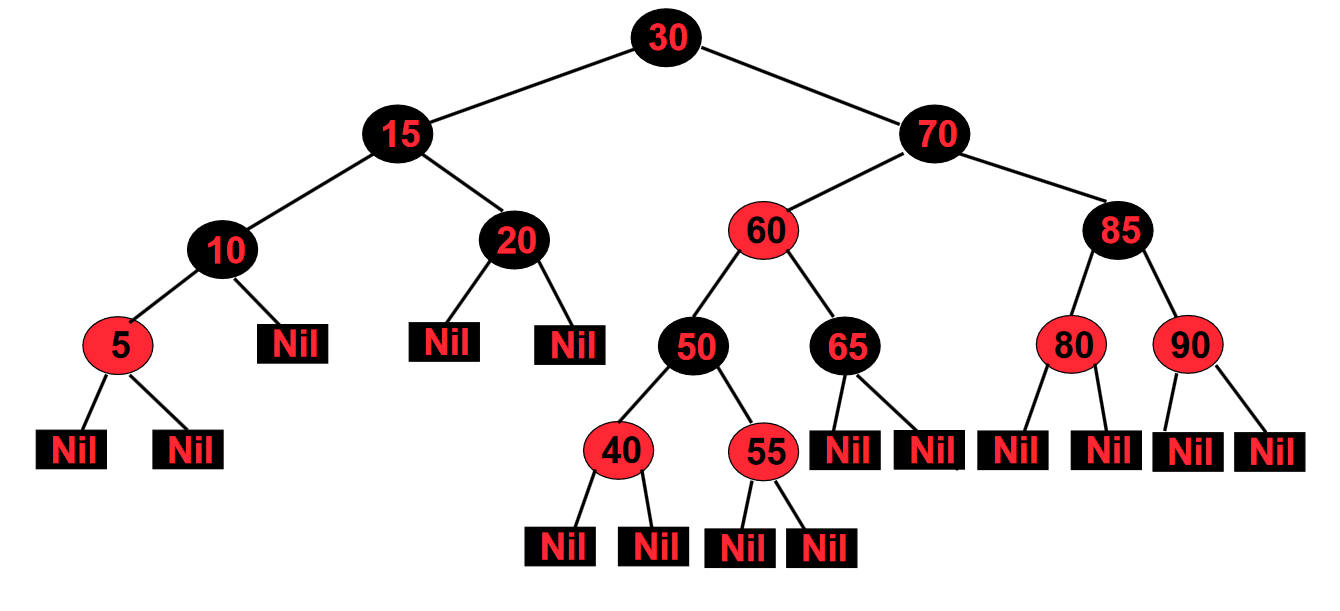
\includegraphics[width=0.5\textwidth]{04/ABR-Red-Black.png}
            \caption{Esempio di albero \textit{Red-Black}}
        \end{figure}
        Se un albero generico è "troppo" sbilanciato, allora potrebbe non rispettare le proprietà di un albero \textit{Red-Black}.
        \begin{figure}
            \centering
            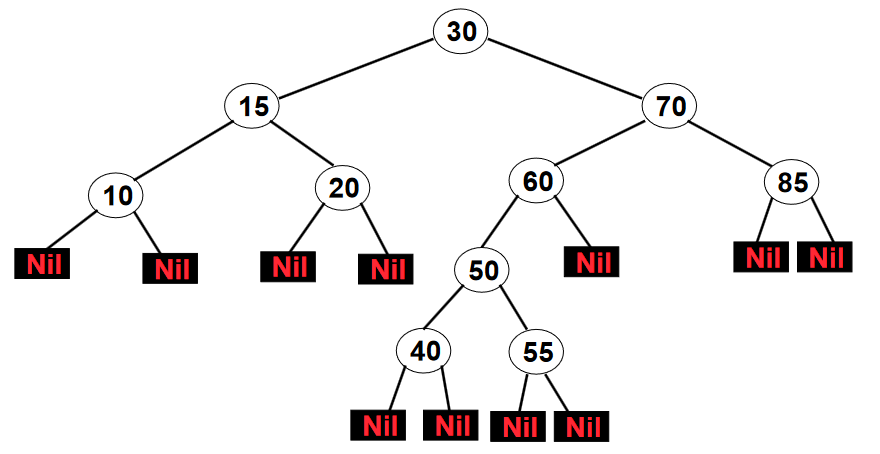
\includegraphics[width=0.5\textwidth]{04/ABR-Red-Black-NotBalanced.png}
            \caption{Esempio di albero non \textit{Red-Black}}
        \end{figure}
    \subsection{Inserimento}
        Quando si và a modificare la struttura dell'albero allora è possibile che determinate condizioni vengano violate, per questo motivo è necessario introdurre delle operazioni di \textbf{ri-bilanciamento} come la \textbf{rotazione} e il \textbf{ri-coloramento}. Le rotazioni a loro volta possono essere di due tipi: \textbf{sinistra} e \textbf{destra}.
        \paragraph{Rotazione a destra}
            \begin{figure}[H]
                \centering
                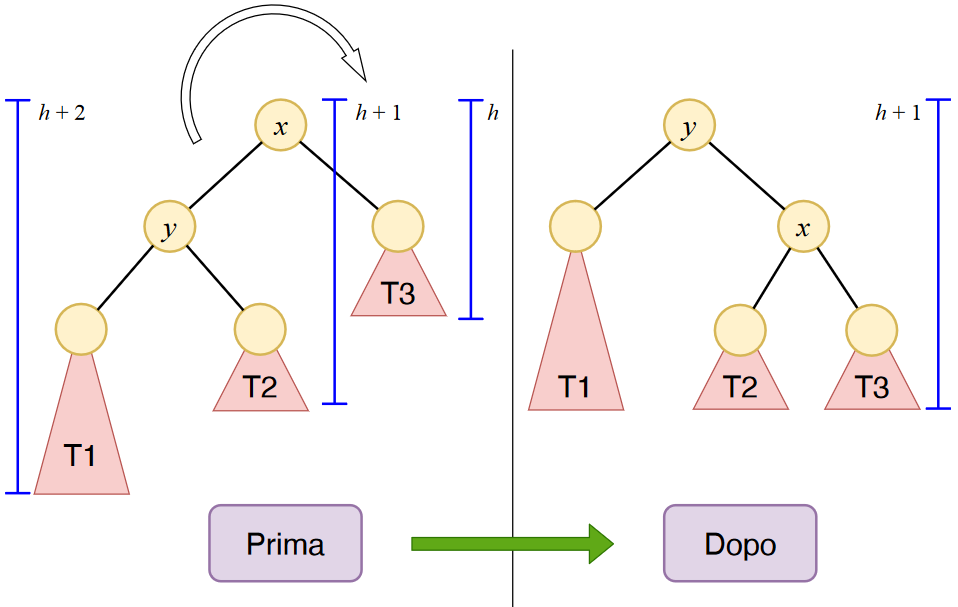
\includegraphics[width=0.3\textwidth]{04/rotazioneDestra.png}
                \caption{Esempio di rotazione a destra}
            \end{figure}
        \newpage
        \paragraph{Rotazione a sinistra}
            Assumiamo che la situazione all'interno del nostro albero di ricerca sia la seguente:

            \begin{wrapfigure}{l}{0.1\textwidth}
                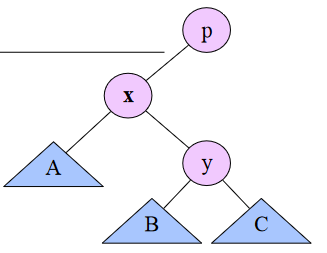
\includegraphics[width=0.9\linewidth]{04/rotazioneSinistra.png}
            \end{wrapfigure}
            Per una rotazione a sinistra si seguono questi passaggi:
            \begin{enumerate}
                \item far diventare $B$ figlio destro di $x$
                \item far diventare $x$ figlio sinistro di $y$
                \item far diventare $y$ figlio di $p$ dove $p$ è il genitore vecchio di $y$
            \end{enumerate}
            Implementazione di tale rotazione:
            \begin{algorithm}[H]
                \caption{rotateLeft(\Tree $ x $)}
                \begin{algorithmic}
                    \State \Tree $ y \gets x.\operatorname{right}()$
                    \State \Tree $ p \gets x.\operatorname{parent}()$
                    \State $ x.\operatorname{right} \gets y.\operatorname{left}()$
                    \If{$ y.\operatorname{left}() \neq \Nil $}
                        \State $ y.\operatorname{left}.\operatorname{parent} \gets x $
                    \EndIf
                    \State $ y.\operatorname{left} \gets x $
                    \State $ x.\operatorname{parent} \gets y $
                    \State $ y.\operatorname{parent} \gets p $
                    \If{$ p \neq \Nil $}
                        \If{$ p.\operatorname{left}() == x $}
                            \State $ p.\operatorname{left} \gets y $
                        \EndIf
                    \EndIf
                    \Return $ y $
                \end{algorithmic}
            \end{algorithm}
        \paragraph{Inserimento in alberi \textit{Red-Balack}}
            Per alberi del genere \textit{Red-Black} l'inserimento di un nodo può violare le proprietà dell'albero, di base inseriamo il nodo come un nodo rosso e eseguiamo il normale inserimento per un albero binario di ricerca. Dopo l'inserimento è necessario verificare se le proprietà n. 3 e n. 4 sono state violate, in tal caso è necessario eseguire delle operazioni di \textbf{ri-bilanciamento}.
            \begin{algorithm}
                \caption{insertNode(\Tree $ T $, \Item $ k $, \Item $ v $)}
                \begin{algorithmic}
                    \State \Tree $ p \gets \Nil $ \Comment{Genitore del nodo da inserire}
                    \State \Tree $ u \gets T $
                    \While{$ u \neq \Nil $ \textbf{and} $u.\operatorname{key}() \neq k $} \Comment{Cerco la posizione del nodo da inserire}
                        \State $ p \gets u $
                        \State $ u \gets \operatorname{iff}(k < u.\operatorname{key}(), u.\operatorname{left}(), u.\operatorname{right}()) $
                    \EndWhile
                    \If{$ u \neq \Nil $ \textbf{and} $u.\operatorname{key}() == k $}
                        \State $ u.\operatorname{value} \gets v $ \Comment{Aggiorno il valore in quanto la chiave è già presente}
                    \Else
                        \State \Tree $ new \gets \New \Item(k, v)$
                        \State \Call{link}{$ p, new, k $}
                        \State \Call{balanceInsert}{$ new $}
                        \If{$ p == \Nil $}
                            \State $ T \gets new $ \Comment{Se il genitore è nullo, allora il nuovo nodo è la radice}
                        \EndIf
                    \EndIf
                    \State \Return $ T $ \Comment{Restituisco l'albero}
                \end{algorithmic}
            \end{algorithm}
            La funzione \texttt{balanceInsert()} è una funzione che si occupa di ri-bilanciare l'albero dopo l'inserimento di un nodo, questa funzione è necessaria in quanto l'inserimento di un nodo potrebbe violare le proprietà dell'albero \textit{Red-Black}.\newline
            Il funzionamento di linea generale prevede: lo spostamento verso l'alto lungo il percorso di inserimento, ripristinare il vincolo dei figli di un nodo rosso che devono essere neri, spostare le violazioni verso l'alto (rotazione) rispettando il vincolo dei nodi neri (ri-coloramento). Terminiamo la funzione con il ri-coloramento della radice se necessario.

            \begin{wrapfigure}{l}{0.3\textwidth}
                \centering
                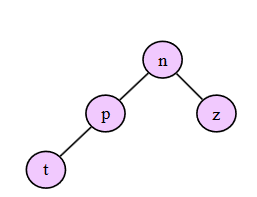
\includegraphics[width=0.3\textwidth]{04/nodiCoinvolti.png}
            \end{wrapfigure}

            I nodi coinvolti ricorsivamente sono i seguenti:

            \begin{itemize}
                \item Il nodo inserito $ t $
                \item Suo padre $ p $
                \item Suo nonno $ n $
                \item Suo zio $ z $
            \end{itemize}
            
            La seguente testata di funzione è comune a tutte le funzioni di ri-bilanciamento:
            \begin{algorithm}[H]
                \caption{balanceInsert(\Tree $ t $)}
                \begin{algorithmic}
                    \State \Tree $ p \gets t.\operatorname{parent}()$
                    \State \Tree $ n \gets \operatorname{iff}(p \neq \Nil, p.\operatorname{parent}(), \Nil)$
                    \State \Tree $ z \gets \operatorname{iff}(n = \Nil, \Nil, \operatorname{iff}(n.\operatorname{left}() == p, n.\operatorname{right}(), n.\operatorname{left}()))$
                \end{algorithmic}
            \end{algorithm}

            É possibile distinguere l'inserimento in 7 casi differenti quali:
            
                \subparagraph{Caso 1}
                
                Nuovo nodo $ t $ non ha padre, dunque è la radice dell'albero. In tal caso, lo coloriamo di nero.
                
                \begin{figure}[H]
                    \centering
                    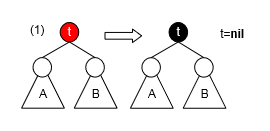
\includegraphics[width=0.3\textwidth]{04/inserimento-1.png}
                    \caption{Nuovo nodo $t$ come radice.}
                \end{figure}
                
                \subparagraph{Caso 2}
                
                Il padre $ p $ di $ t $ è nero; in tal caso, non c'è nessuna violazione delle proprietà dell'albero \textit{Red-Black} e inseriamo il nodo $ t $ come nodo rosso.                
                \begin{figure}[H]
                    \centering
                    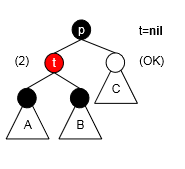
\includegraphics[width=0.3\textwidth]{04/inserimento-2.png}
                    \caption{Il padre $p$ di $t$ è nero.}
                \end{figure}
                \subparagraph{Caso 3}
                    Caso in cui l'elemento da inserire sia rosso e il padre sia rosso e lo zio sia rosso. Coloriamo dunque $ p $ e $ z $ di nero e $ n $ di rosso (l'altezza nera rimane invariata).
                    La problematica ora sorge sul nonno $ n $ che potrebbe violare le proprietà 1 e/o 3 dell'albero \textit{Red-Black}, in tal caso dobbiamo eseguire una ricorsione su $ n $ ponendo $ t = n $ e ripetendo il processo.
                    \begin{figure}[H]
                        \centering
                        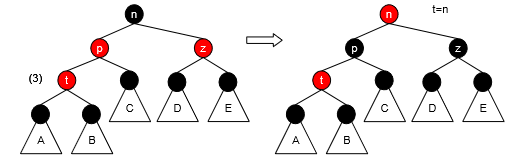
\includegraphics[width=0.6\textwidth]{04/inserimento-3.png}
                    \end{figure}
                \subparagraph{Caso 4 (a,b)}
                    In questo caso $ t $ è rosso, $ p $ è rosso e $ z $ è nero. Questo caso si divide in due sotto-casi ma il procedimento è speculare per entrambi (sostituendo $ left $ con $ right $ e viceversa).\newline
                    Assumendo che $ t $ sia figlio \underline{destro} di $ p $ e che $ p $ sia figlio \underline{sinistro} di $ n $, allora eseguiamo una rotazione a \underline{sinistra} su $ p $ in modo da rendere $ t $ figlio sinistro di $ n $ con $ p $ come figlio sinistro di $ t $. Ora abbiamo una violazione delle proprietà 3 e 4. Ricadiamo però nel caso 5(a) in quanto $ p $ è figlio \underline{sinistro} di $ n $ e $ t $ è figlio \underline{sinistro} di $ p $.
                    \begin{figure}[H]
                        \centering
                        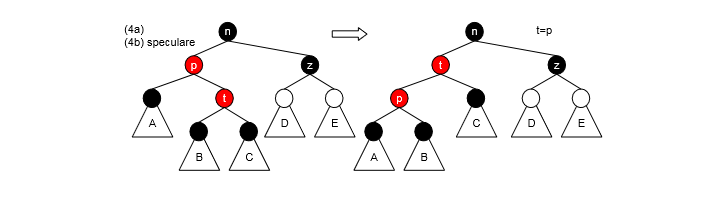
\includegraphics[width=0.9\textwidth]{04/inserimento-4.png}
                    \end{figure}
                \subparagraph{Caso 5 (a,b)}
                    In questo caso $ t $ è rosso, $ p $ è rosso e $ z $ è nero. Questo caso si divide in due sotto-casi, come il precedente, ma il procedimento è speculare per entrambi (sostituendo $ left $ con $ right $ e viceversa).\newline
                    Assumendo che $ t $ sia figlio \underline{sinistro} di $ p $ e che $ p $ sia figlio \underline{sinistro} di $ n $, allora eseguiamo una rotazione a \underline{destra} su $ n $ in modo da rendere $ p $ nodo radice, $ t $ figlio sinistro di $ p $ e $ n $ figlio destro di $ p $. Ora coloriamo $ p $ di nero e $ n $ di rosso. In quando la posizione relativa di $ z $ rispetto a $ n $ non cambia allora i vincoli per l'albero \textit{Red-Black} sono rispettati.
                    \begin{figure}[H]
                        \centering
                        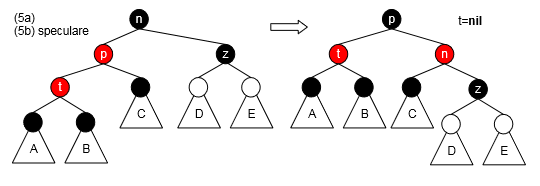
\includegraphics[width=0.6\textwidth]{04/inserimento-5.png}
                    \end{figure}
                \subparagraph{Conclusioni}
                    I casi 1 e 2 non richiedono ulteriori operazioni, i casi 3, 4 e 5 richiedono una rotazione e un ri-coloramento (con eventuali ricorsioni). In generale, l'inserimento di un nodo in un albero \textit{Red-Black} richiede $O(\log n)$ operazioni. É implementabile con il seguente pseudo-codice:
                    \newpage
                    \begin{algorithm}
                        \caption{balanceInsert(\Tree $ t $)}
                        \begin{algorithmic}
                            \State $ t.\operatorname{color} \gets \text{RED} $
                            \While{$t\neq \Nil $}
                                \State \Tree $ p \gets t.\operatorname{parent}()$
                                \State \Tree $ n \gets \operatorname{iff}(p \neq \Nil, p.\operatorname{parent}(), \Nil)$
                                \State \Tree $ z \gets \operatorname{iff}(n = \Nil, \Nil, \operatorname{iff}(n.\operatorname{left}() == p, n.\operatorname{right}(), n.\operatorname{left}()))$
                                \If{$ p = \Nil $} \Comment{Caso 1}
                                    \State $ t.\operatorname{color} \gets \text{BLACK} $
                                    \State $ t \gets \Nil $
                                \ElsIf{$ p.\operatorname{color} == \text{BLACK} $} \Comment{Caso 2}
                                    \State $ t \gets \Nil $
                                \ElsIf{$ z.\operatorname{color} == \text{RED} $} \Comment{Caso 3}
                                    \State $ p.\operatorname{color} \gets \text{BLACK} $
                                    \State $ z.\operatorname{color} \gets \text{BLACK} $
                                    \State $ n.\operatorname{color} \gets \text{RED} $
                                    \State $ t \gets n $
                                \Else
                                    \If{$ t == p.\operatorname{right}() \textbf{and} p == n.\operatorname{left}() $} \Comment{Caso 4.a}
                                        \State \Call{rotateLeft}{$ p $}
                                        \State $ t \gets p $
                                    \ElsIf{$ t == p.\operatorname{left}() \textbf{and} p == n.\operatorname{right}() $} \Comment{Caso 4.b}
                                        \State \Call{rotateRight}{$ p $}
                                        \State $ t \gets p $
                                    \Else
                                        \If{$ t == p.\operatorname{left}() \textbf{and} p == n.\operatorname{left}() $} \Comment{Caso 5.a}
                                            \State \Call{rotateRight}{$ n $}
                                        \ElsIf {$ t == p.\operatorname{right}() \textbf{and} p == n.\operatorname{right}() $} \Comment{Caso 5.b}
                                            \State \Call{rotateLeft}{$ n $}
                                        \EndIf
                                        \State $ p.\operatorname{color} \gets \text{BLACK} $
                                        \State $ n.\operatorname{color} \gets \text{RED} $
                                    \EndIf
                                \EndIf
                            \EndWhile
                        \end{algorithmic}
                    \end{algorithm}
    \subsection{Teoremi su un albero \textit{Red-Black}}
        \begin{theorem}
            In un albero \texttt{RB}, un sotto-albero di radice $ u $ contiene $ n \geq 2^{\operatorname{bh(u)}} - 1 $ nodi interni (nodi senza foglie fittizie).
        \end{theorem}
        \begin{proof}
            Si procede per ricorsione sull'altezza dell'albero:\newline
            \textbf{Base:} se $ h=0$ allora $ u $ è una foglia \textbf{Nil} e il sotto-albero con radice $ u $ contiene: $n\geq 2^{\operatorname{bh}(u)} - 1 = 2^0 - 1 = 0$ nodi interni.\checkmark\newline
            \textbf{Passo:} supponendo che $ h > 1 $ e che la tesi sia vera per alberi di altezza $ < h $, Allora $ u $ è un nodo interno con due figli non fittizi. Inoltre ogni figlio $ v $ di $ u $ ha un'altezza nera $ \operatorname{bh}(v) $ pari a $ \operatorname{bh}(u) $ se v è rosso o $ \operatorname{bh}(u) - 1 $ se $ v $ è nero. Quindi il sotto-albero con radice $ v $ contiene almeno $ 2^{\operatorname{bh}(v)} - 1 $ nodi interni, per ipotesi induttiva. In quanto considerando anche il nodo $ u $, allora il numero di nodi interni nel sotto-albero con radice $ u $ è almeno $ n\geq 2\cdot \left(2^{\operatorname{bh}(v)} - 1\right) + 1 = 2^{\operatorname{bh}(u)} - 2 + 1 = 2^{\operatorname{bh}(u)} - 1 $.\checkmark
        \end{proof}
        \begin{theorem}
            In un albero \texttt{RB}, almeno la metà dei nodi dalla radice ad una foglia sono neri.
        \end{theorem}
        \begin{proof}
            Per il vincolo (2) di un albero \texttt{RB}, se un nodo è rosso allora i suoi figli devono essere neri. Quindi la situazione nella quale si ottengono più nodi rossi possibili è nel caso questi siano con colori alterni.\newline
            Quindi almeno la metà dei nodi dalla radice ad una foglia sono neri.
        \end{proof}
        \begin{theorem}
            In un albero \texttt{RB} dati due cammini dalla radice a due foglie non è possibile che un uno sia più lungo del doppio dell'altro.
        \end{theorem}
        \begin{proof}
            Per il vincolo (4) di un albero \texttt{RB}, ogni cammino dalla radice ad una foglia deve avere lo stesso numero di nodi neri. Per il teorema precedente almeno la metà dei nodi in ognuno di questi cammini sono neri.\newline
            Quindi al limite uno dei due cammini è costituito solo da nodi neri e l'altro è costituito da nodi alternati neri e rossi, rendendo la lunghezza del cammino con nodi alternati esattamente il doppio del cammino con nodi neri per (4).
        \end{proof}
        \begin{theorem}
            L'altezza massima di un albero \texttt{RB} con $ n $ nodi è al più $ 2\log(n+1) $.
        \end{theorem}
        \begin{proof}
            $$
                \begin{aligned}
                    n\geq 2^{\operatorname{bh}(r)} -1 &\Leftrightarrow \overbrace{n\geq 2^{\frac{h}{2}}}^{\operatorname{bh}(r)\leq \frac{h}2} - 1\\
                    & \Leftrightarrow n+1\geq 2^{\frac{h}{2}}\\
                    & \Leftrightarrow \log(n+1)\geq \frac{h}{2}\\
                    & \Leftrightarrow 2\log(n+1)\geq h
                \end{aligned}
            $$
        \end{proof}
        Dunque conseguenza di questo teorema è che la complessità totale di un albero \texttt{RB} è $O(\log n)$, in quanto:
        \begin{enumerate}
            \item $O(\log n)$ per scendere fino al punto di inserimento del nodo
            \item $O(1)$ per inserire il nodo
            \item $O(\log n)$ per risalire e ri-bilanciare l'albero (caso peggiore caso: 3)
        \end{enumerate}
    \subsection{Cancellazione}
        La cancellazione di un nodo in un albero \textit{Red-Black} è più complessa rispetto all'inserimento, in quanto la cancellazione di un nodo potrebbe violare le proprietà dell'albero. La procedura di cancellazione è simile a quella di un albero binario di ricerca, ma con delle operazioni di ri-bilanciamento. La procedura di cancellazione è composta da 8 casi differenti, con 4 casi principali e 4 casi simmetrici.\newline
        In generale:
        \begin{itemize}
            \item Se il nodo da eliminare è rosso allora:
                \subitem Altezza nera invariata
                \subitem Non sono stati creati nodi rossi consecutivi
                \subitem La radice resta nera
            \item Se il nodo da eliminare è nero allora:
                \subitem Potrebbe essere violato il vincolo 1 in quanto la radice potrebbe essere diventata rossa
                \subitem Potrebbe essere violato il vincolo 3 in quanto potrebbero esserci nodi rossi consecutivi se padre e figlio sono rossi
                \subitem Potrebbe essere violato il vincolo 4 in quanto l'altezza nera è diminuita
        \end{itemize}
        \begin{algorithm}[H]
            \caption{balanceDelete(\Tree $ T $, \Tree $ t $)}
            \begin{algorithmic}
                \While{$t\neq  \textbf{and } t.\operatorname{color}()=\text{black}$}
                    \State \Tree $ p \gets t.\operatorname{parent}()$ \Comment{Ottengo il genitore del nodo da eliminare}
                    \If{$t=p.\operatorname{left}() $} \Comment{Sottocasi con $t$ figlio sinistro}
                        \State \Tree $f \gets p.\operatorname{right}()$ \Comment{Ottengo il fratello del nodo da eliminare}
                        \State \Tree $ns \gets f.\operatorname{left}()$ \Comment{Ottengo il nipote sinistro del fratello}
                        \State \Tree $nd \gets f.\operatorname{right}()$ \Comment{Ottengo il nipote destro del fratello}
                        \If{$f.\operatorname{color}()=\text{red}$} \Comment{Caso 1}
                            \State $p.\operatorname{color} \gets \text{red}$
                            \State $f.\operatorname{color} \gets \text{black}$
                            \State \Call{rotateLeft}{$p$}
                        \Else
                            \If{$ns.\operatorname{color}()=\text{black} \textbf{ and } nd.\operatorname{color}()=\text{black}$} \Comment{Caso 2}
                                \State $f.\operatorname{color} \gets \text{red}$
                                \State $t \gets p$
                            \ElsIf{$ns.\operatorname{color}()=\text{red} \textbf{and} nd.\operatorname{color}()=\text{black}$} \Comment{Caso 3}
                                \State $ns.\operatorname{color} \gets \text{black}$
                                \State $f.\operatorname{color} \gets \text{red}$
                                \State \Call{rotateRight}{$f$}
                            \ElsIf{$nd.\operatorname{color}()=\text{red}$} \Comment{Caso 4}
                                \State $f.\operatorname{color} \gets p.\operatorname{color}()$
                                \State $p.\operatorname{color} \gets \text{black}$
                                \State $nd.\operatorname{color} \gets \text{black}$
                                \State \Call{rotateLeft}{$p$}
                                \State $t \gets T$
                            \EndIf
                        \EndIf
                    \Else
                        \State \Comment{Sottocasi con $t$ figlio destro, tralasciati in quanto simmetrici}
                    \EndIf
                \EndWhile
            \end{algorithmic}
        \end{algorithm}
        Dunque seppure complicata la cancellazione risulta efficiente in quanto:
        \begin{itemize}
            \item Dal caso (1) si passa ad uno dei casi (2,3,4)
            \item Dal caso (2) si risale ad uno degli altri casi, ma si risale di un livello
            \item Dal caso (3) si passa al caso (4)
            \item Nel caso (4) si termina
        \end{itemize}
        La complessità totale di una cancellazione in un albero \textit{Red-Black} è $O(\log n)$.